\documentclass{article} 
\usepackage[left=0.75in,top=0.6in,right=0.75in,bottom=0.6in]{geometry} % Document margins
\usepackage{tabularx}
\usepackage{fancyvrb}
\usepackage{graphicx}
\usepackage{multicol,caption}
\usepackage{fancyhdr}
\usepackage{lipsum}
\usepackage{mathtools}
\usepackage{float}
\usepackage{textcomp}

%Header Stuff
\newenvironment{Figure}
  {\par\medskip\noindent\ignorespaces\minipage{\linewidth}}
  {\endminipage\par\medskip}

\usepackage{fancyhdr}
\pagestyle{fancy}
\fancyhf{}
\renewcommand{\headrulewidth}{0pt}
\fancyhead[R]{\thepage}


\begin{document}

%----------------------------------------------------------------------------------------
%		 TITLE 
%----------------------------------------------------------------------------------------
\begin{center}

\vspace* {15 pt}
\Huge{\bf Establishing communication between Qt program and DE2-115 FPGA }\\
\vspace {20 pt}
\large{Howard Edwards, Michael Micros, Jonathon  Rigney, Megan Rowland \\}

\end{center}

\vspace{15 pt}




\begin{multicols*}{2}

%----------------------------------------------------------------------------------------
%		ABSTRACT
%----------------------------------------------------------------------------------------
{\bf  \textit {Abstract(Jonathon Rigney)} ---}
\par This report is only part of a series of papers aimed at designing and implementing a system to perform real time video processing using a Field Programmable Gate Array(FPGA) controlled by a Graphical User Interface(GUI). This paper deals specifically with establishing communication between Qt and the DE2-115 FPGA. The slider value from a Qt GUI program was succesfully transferred to the FPGA via RS232 serial communication. The design makes use of the QSerialPort Class on the Qt side, in order to be able to send the slider value one character at a time over the RS232 connection. On the FPGA side, a NIOS II (Basic Computer) processor is programmed onto the board making additional use of a C program. The C program receives the characters sent from the Qt program, and displays the values on 2 7-segment displays on the DE2-115 FPGA.


{\bf  \textit {Index Terms} --- FPGA, 8-bit counter, Seven Segment Display}



%----------------------------------------------------------------------------------------
%		INTRODUCTION
%----------------------------------------------------------------------------------------

\begin{center}
\large{I. Introduction(Howard Edwards)}
\end{center}
\par This report documents the goal to establish communication between a graphical user-interface, GUI, and a field-programmable gate array, FPGA,  board. This goal was a fraction of an integrated system that performs the processing of real-time video through an user-interface on a computer and the use of FPGAs. The GUI was developed with Qt cross-platform application, and the FPGA board was the Altera DE2- 115. Both the Qt GUI creation and the Altera DE2-115 familiarization was discussed in another report by Edwards, Micros et al.

    Communication was established between the GUI and FPGA through RS232. The GUI sends data to the computer’s RS232 port which is then receive by the DE2-115 boards via its RS232 interface. In order for the board to receive this data, a basic computer called the DE2 Basic Computer was programmed onto the FPGA. One of its main component is the Altera Nios II processor. In order to assemble and compile Nios II programs, written in C programming language or assembly, the Altera Monitor program was utilized.

   The program was written in C programming language to program Nios II. The program allows for the value of the brightness slider in the GUI to be received from the RS232 interface and displayed onto the board’s 7-segment display. Before this was accomplished, the RS232 library was implemented onto the Qt application to send the slider’s value to the computer's port to be received. With both Qt  and Nios II written programs running in unison, communication between GUI and the FPGA board operated as desired.\\



%----------------------------------------------------------------------------------------
%		DESIGN
%----------------------------------------------------------------------------------------
\vspace{10 pt}
\begin{center}
{\large II. Design (Michael Micros)}
\end{center}

{\bf A. Summary of Design--}  
The overall design aims at achieving communication between a Qt program and a DE2-115 Altera FPGA. More specifically, we attempt to send a slider value used in a GUI over an RS232 port, in order to display the value on 2 7-segment LEDs of the FPGA. To achieve this minor modification needed to be made to pre-existing code from a previous paper by Edwards et al that implements a GUI that allows the user to adjust the brightness and contrast of an image. Additionally, code was written to read from the RS232 port of the FPGA and display the received digits.\\

{\bf B. Detail Description}\\
{\bf Qt Design:} 
In order to establish communication through the QT GUI and the RS232 serial port, the QSerialPort Class, provided by QT, is utilized. The RS232 serial port on the computer utilized for this project is named com1 and is configured as com1 in the QT program. For the RS232 serial port, the correct baud rate, data bits, parity, and stop bits need to be configured in the mainwindow.cpp file of the QT program to transmit data to the Altera board. The RS232 serial port is configured for a baud rate of 115,200, 8-bit data, odd parity, and one stop bit. These settings need to be mirrored in the QT program for correct transmission of data. If any of the values are not configured correctly, the data will be garbled on the receiving end. The settings are added to the initialization of the MainWindow function in mainwindow.cpp file of the QT program to open and configure and connection to the RS232 serial port. The corresponding code can be seen in Fig. 1.



After the connection to the RS232 serial port is opened and configured, the value obtained by the change in the brightness slider is transmitted to the Altera board. In order to do this, code is added to the function called when the brightness slider is moved to the left or right, on\_brightnessSlider\_valueChanged(int value). The value transmitted needs to be in the form of a const char. Also, the value transmitted needs to be two digits, so a zero is added to all of the single digit values before converting. To add the ‘0’ digit we use the Qstring.insert() function that takes as parameters the position to which to add the QChar, and the QChar to be inserted. This will allow the receiving end to display the value on the 7-segment displays correctly. The value from the brightness slider is converted from an integer to a const char and transmitted through the RS232 serial port. The corresponding code can be seen in Fig. 2. \\


\begin{Figure}
 \centering
 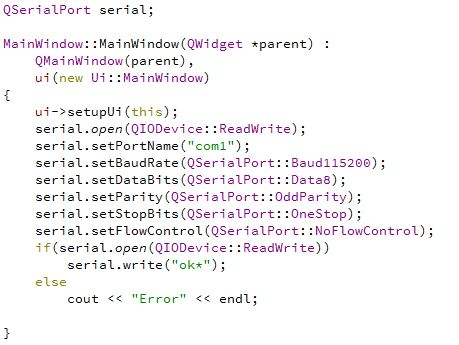
\includegraphics[width=\linewidth,height=5 cm]{mainwindowfunction.JPG}
  \captionof{figure}{C++ code to open and configure the RS232 serial port}
\end{Figure}

\vspace{20 pt}

\begin{Figure}
 \centering
 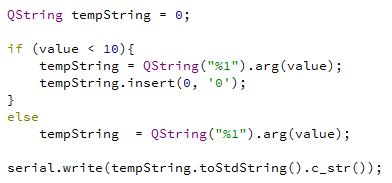
\includegraphics[width=\linewidth]{integertoconstcharsend.JPG}
  \captionof{figure}{C++ code to translate and send a value through the RS232 serial port}
\end{Figure}

\vspace{20 pt}

{\bf Nios II (C) program:} \\
The Nios II design consists of a project created in the Altera Monitor Program that imports a pre written C program and loads it onto the FPGA board. The C code runs in an infinite while loop and performs 3 basic tasks. 1) It listens on the RS232 port for incoming data. 2) When data is received, it outputs it to the console (for testing and confirmation). 3)Sets the appropriate values to the LEDs on the board.

	The RS232 port is referred to in the Nios II by the address of the port which is 0x10001010. In the while loop, we read bit 15 of the value located in the address. This bit is called RVALID and represents whether data is ready to be accessed.  The incoming data(characters) are stored in a FIFO stack and accessed one at a time by reading the 0-7 bits of the aforementioned address.

	Once a digit is read, it is displayed on the Altera Monitor Program console by writing to the 0-7 byte of the JTAG UART port located in address 0x10001000.
	The final task required was displaying the received value (2 characters) on the 7-segment LEDs. In order to be able to distinguish which bit was the first bit and which was the second, an int variable was used to keep track of this. The variable would toggle between 1 and 2. In each cycle through the while loop, the value of the variable would be checked in an if statement, and the flow of the program would shift to the appropriate part of code. The first (most significant digit) character is displayed on LED HEX1, which is done by assigning the digit to the value of   address 0x10000021. The digit is copied to an int variable dig1 for reasons explained later.

	When we receive the second digit, the code enters the appropriate part of the program where the LED HEX0 is given the appropriate value, by assigning the proper 7 bit vector to address 0x10000020. Because LED HEX0 and HEX1 are adjacent byte values, during testing we noticed that when writing to HEX0, HEX1 would be cleared (we assume it was filled with 0s appended to HEX0 because we are not writing an 8-bit value but a 32 bit value probably). That is the purpose on variable dig1 introduced earlier. After writing to HEX0 we rewrite HEX1.

	The C code that performs the previous tasks is included in the Appendix.




%----------------------------------------------------------------------------------------
%		EVALUATION
%----------------------------------------------------------------------------------------

\begin{center}
{\large III. Evaluation (Megan Rowland)}\\
\end{center}

The implemented design performed as designed. When running the GUI from QT, a user will select an image. When adjusting the brightness of that image, the value from the brightness slider will be transmitted through the RS232 serial port to the Altera board via the DE2-115 basic computer. When the DE2-115 basic computer receives the value it will then write that value to the correct 7-segment display. The most significant digit will be written to the left 7-segment display and the least significant digit will be written to the right 7-segment display. If the value from the brightness slider is a single digit, the value will be transmitted as two digits with a leading zero and the value viewed on the 7-segment display will be a zero written to the left 7-segment display and the single digit written to the right 7-segment display. Every time the brightness slider is moved, the value on the 7-segment display updates:

\begin{Figure}
 \centering
 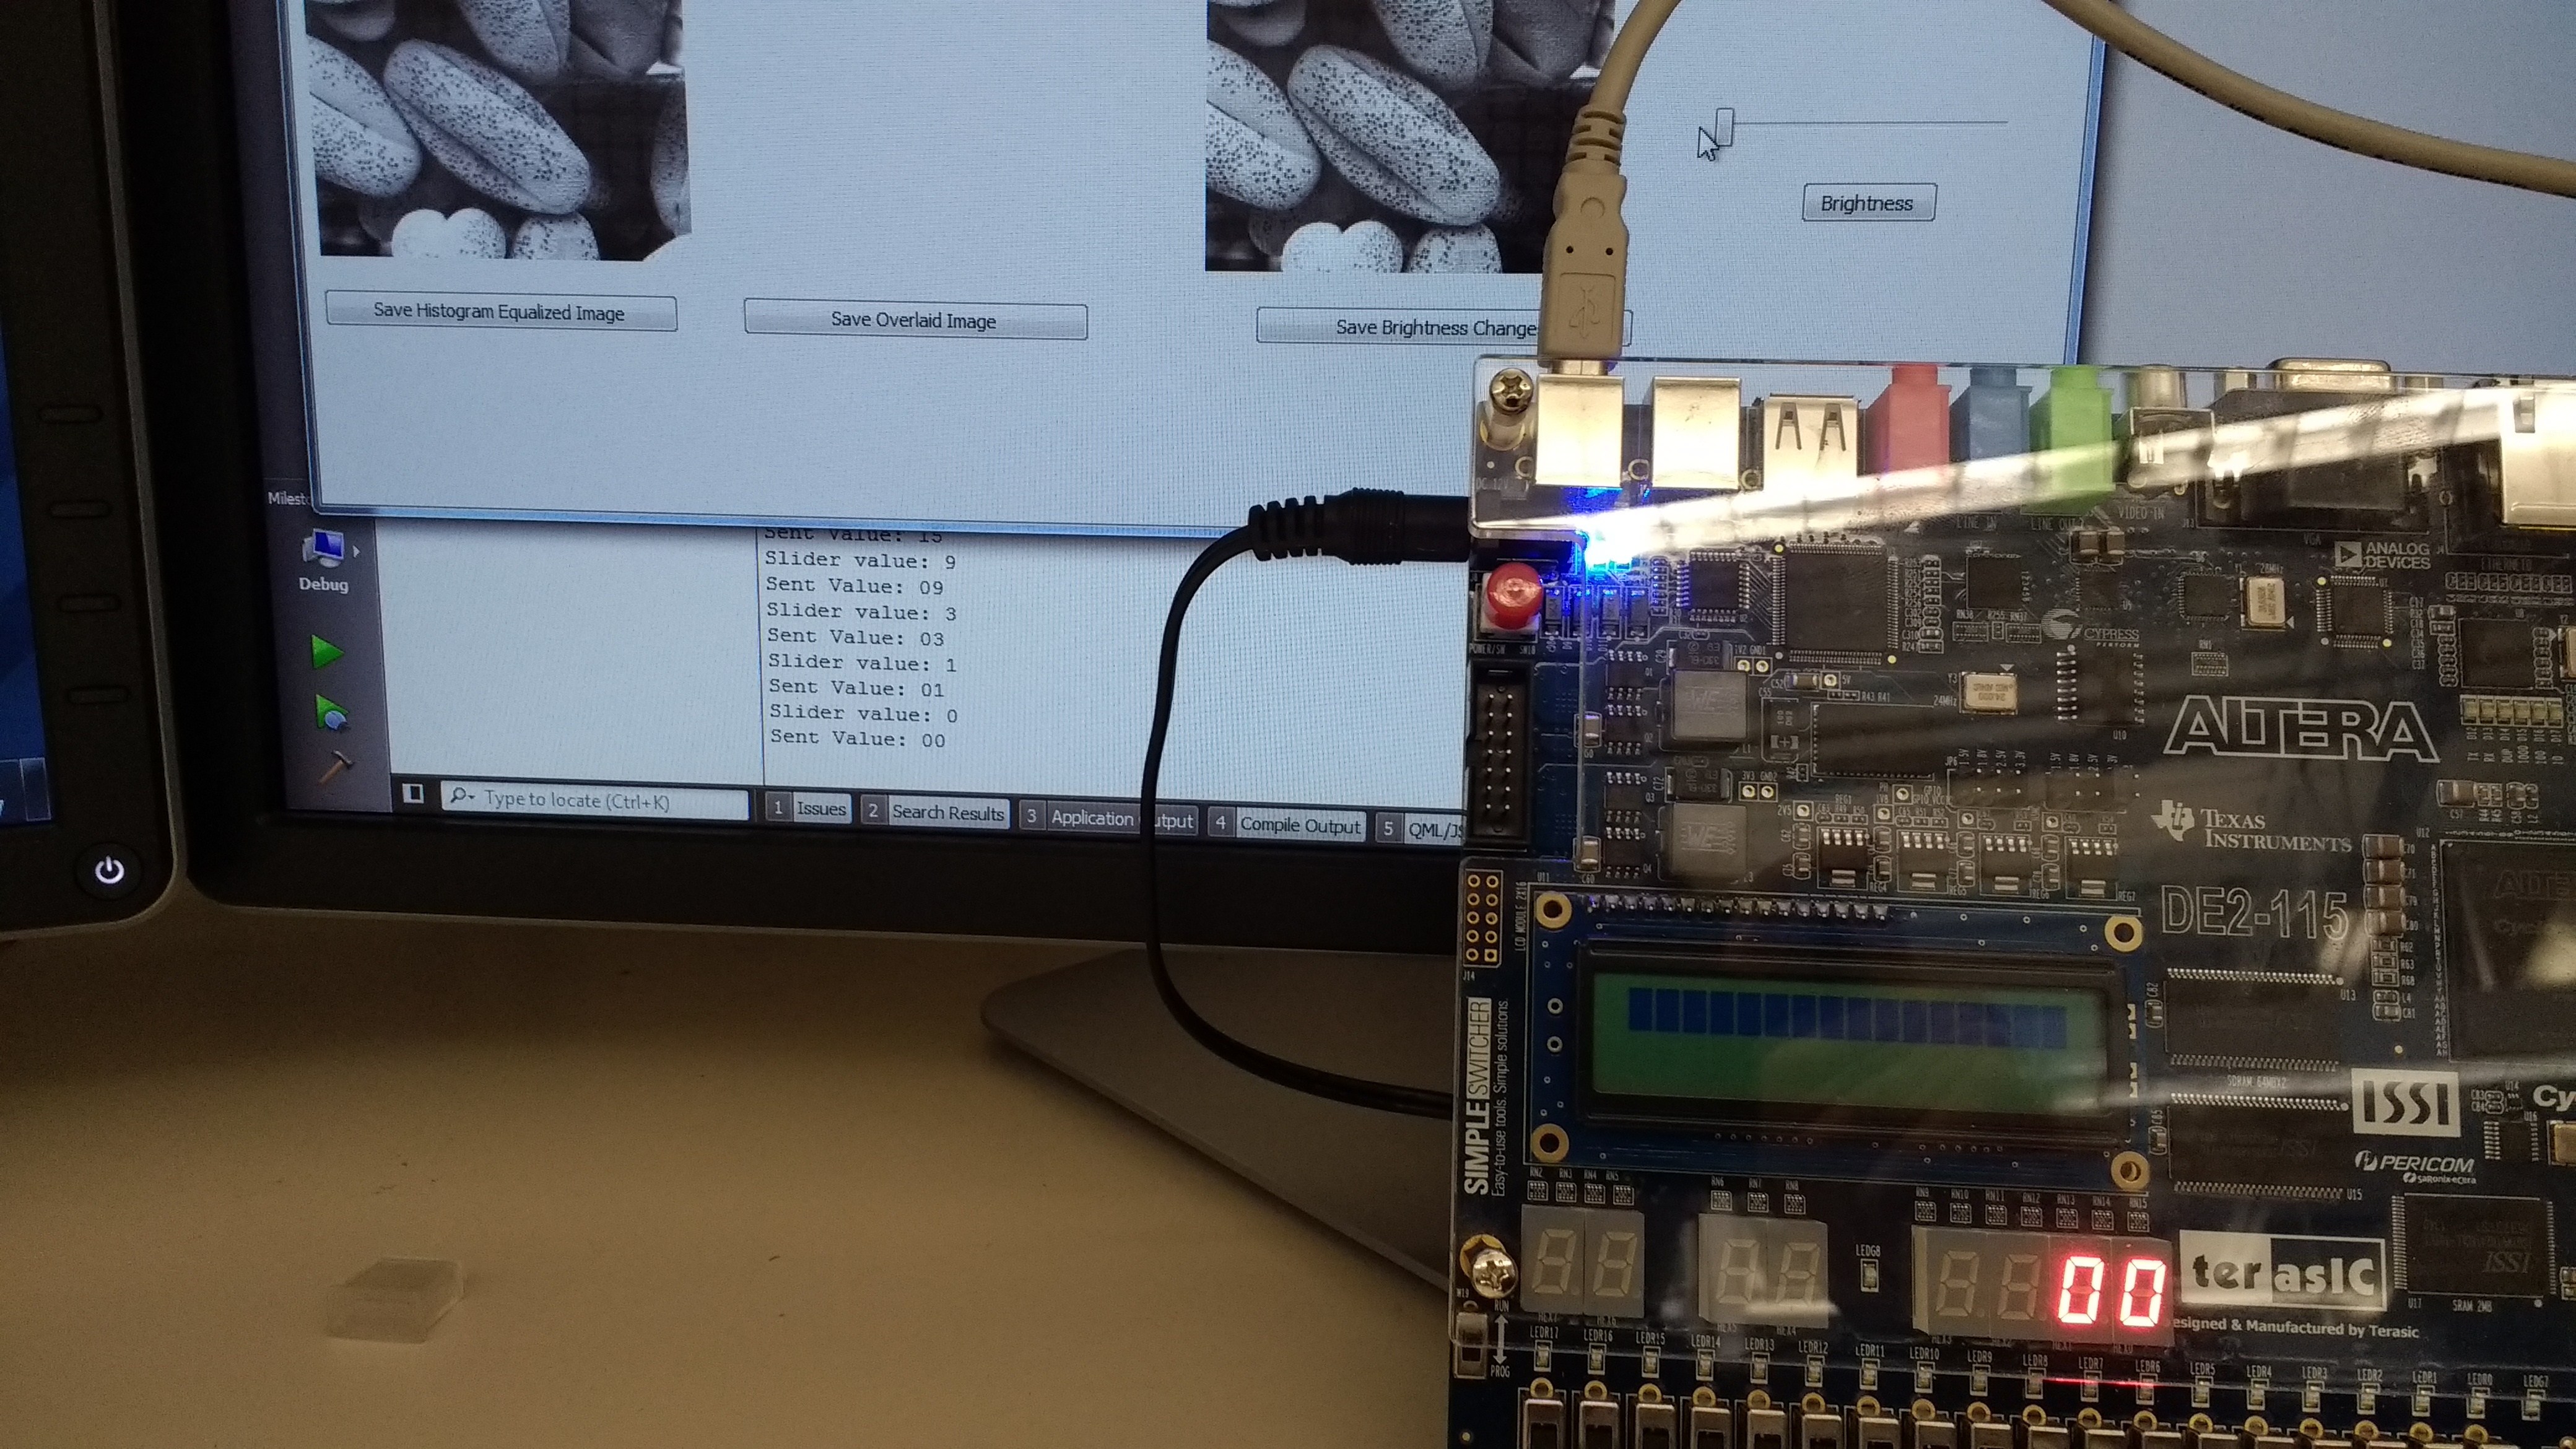
\includegraphics[width=\linewidth]{display_00.JPG}
  \captionof{figure}{Brightness slider moved down to 0}
\end{Figure}

\begin{Figure}
 \centering
 \includegraphics[width=\linewidth]{display_49.JPG}
  \captionof{figure}{Brightness slider moved to 49}
\end{Figure}

\begin{Figure}
 \centering
 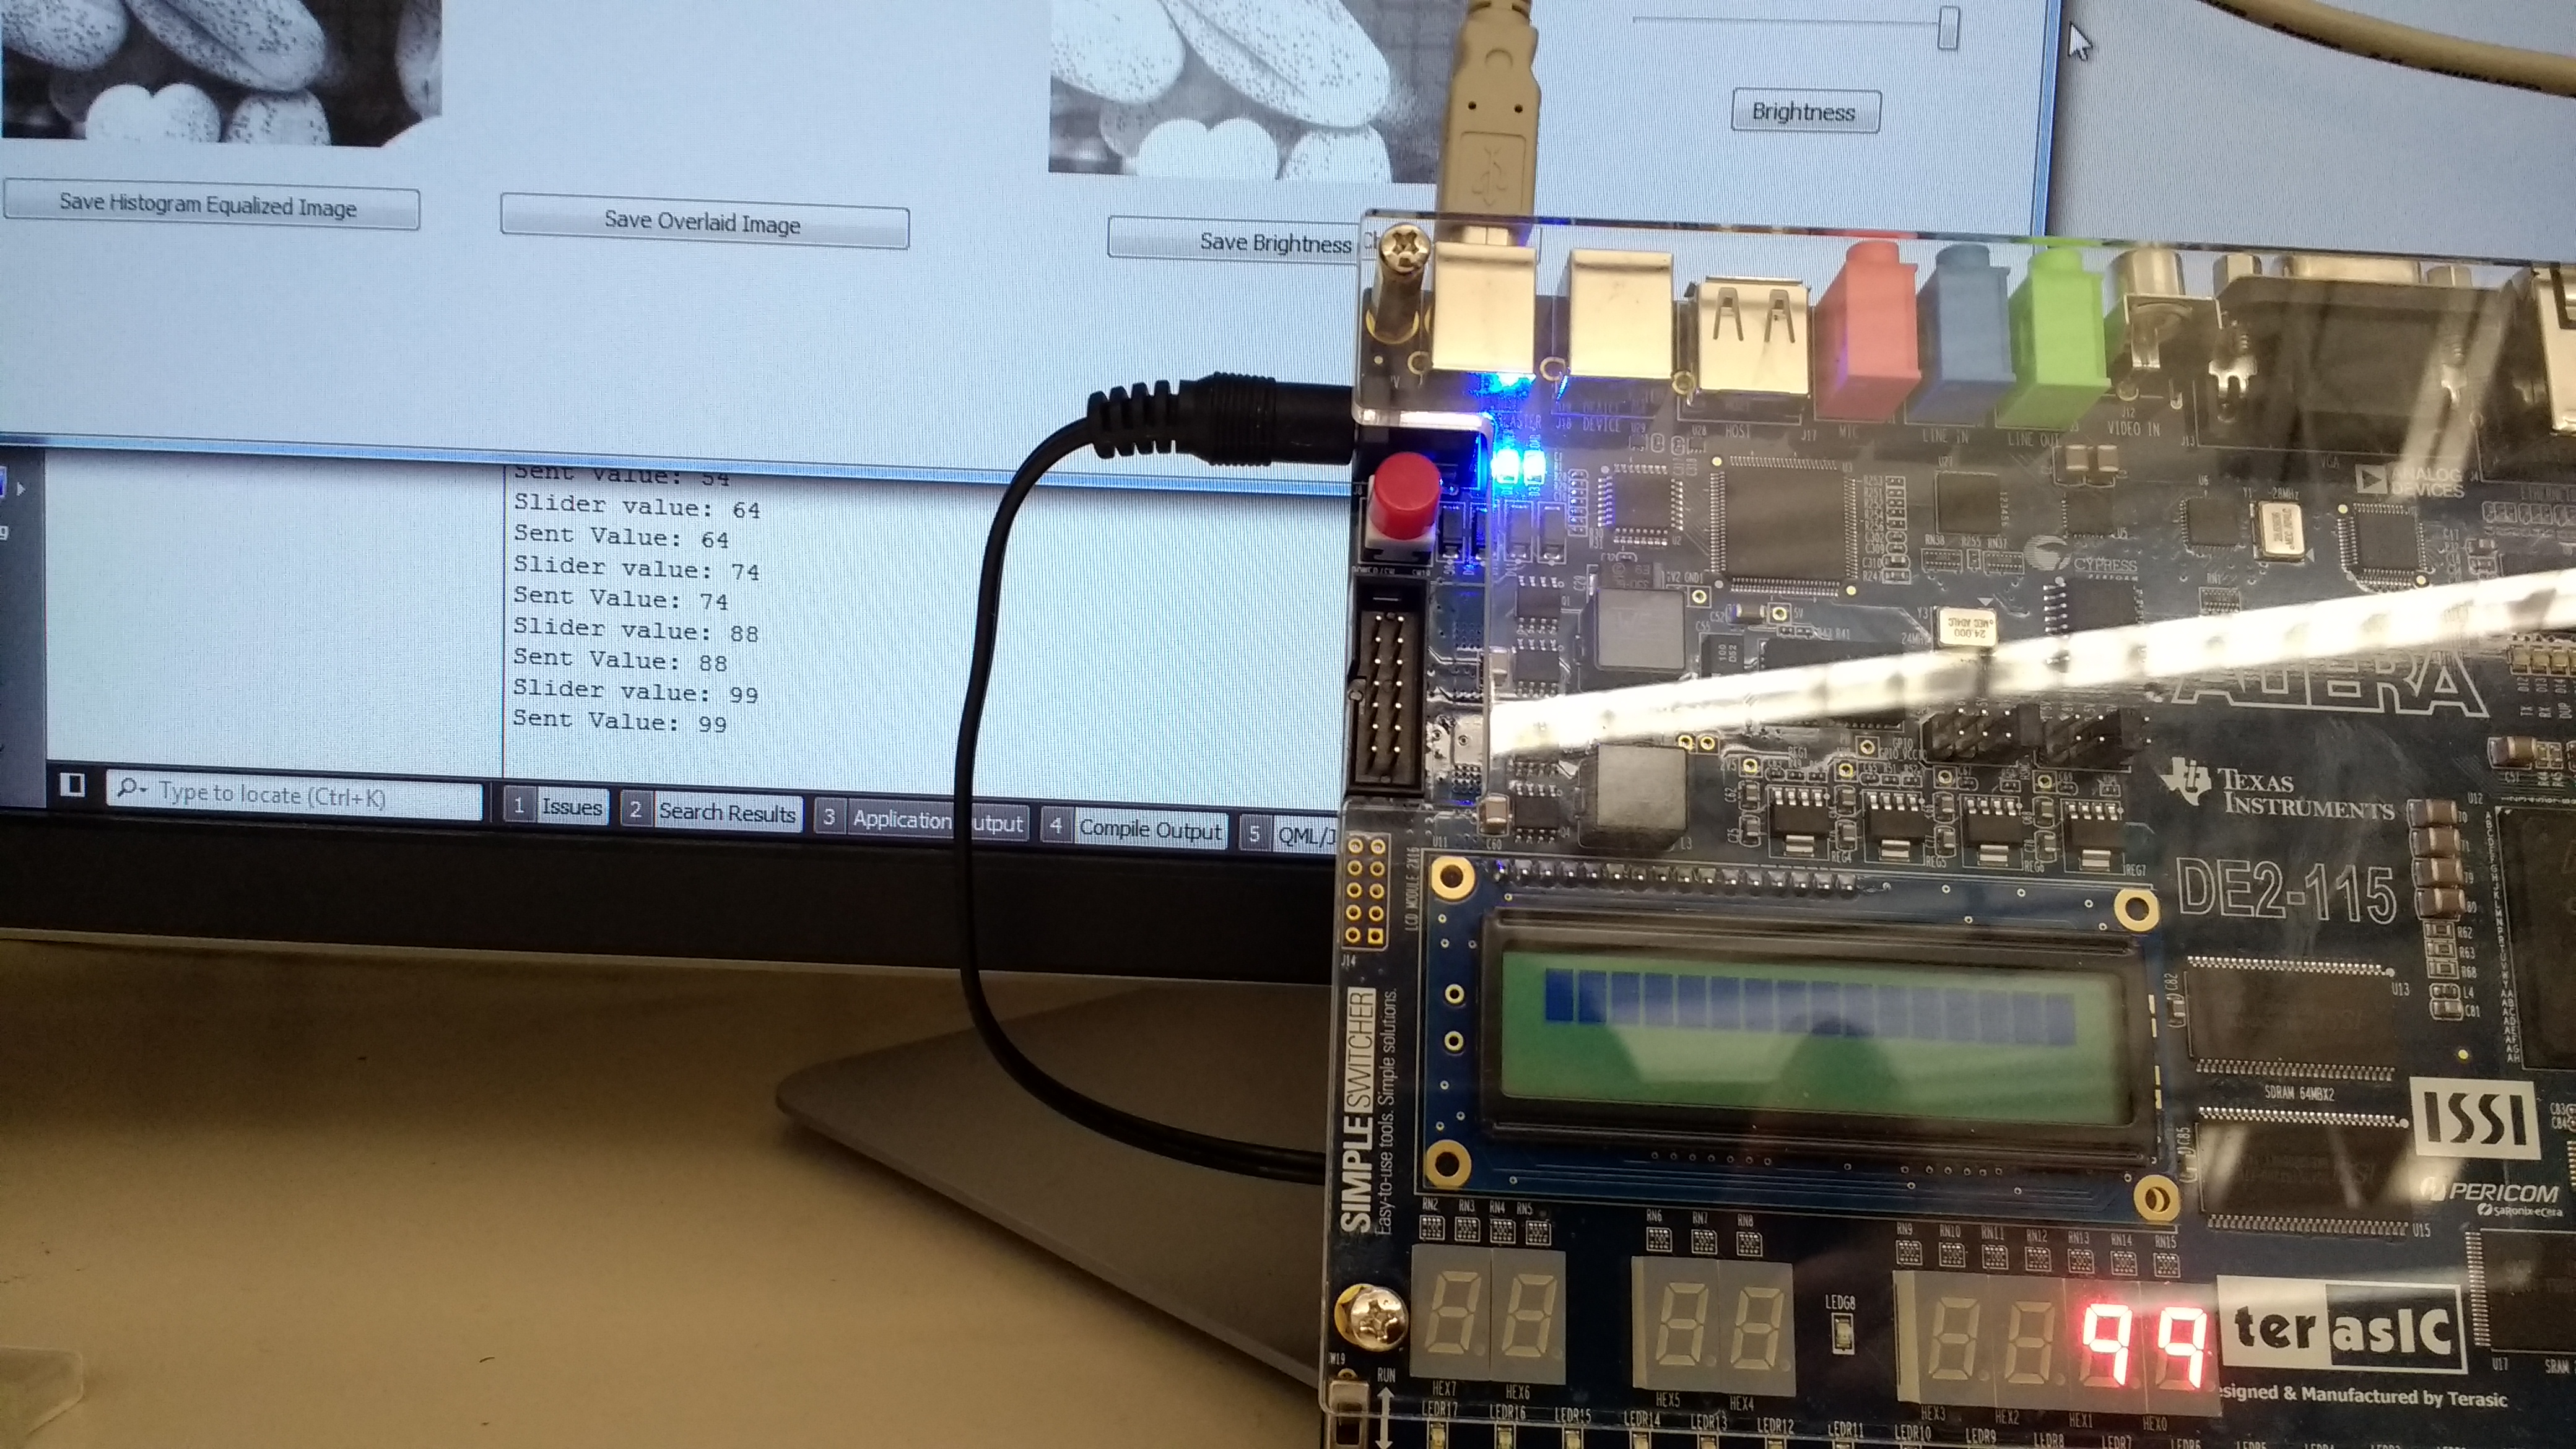
\includegraphics[width=\linewidth]{display_99.JPG}
  \captionof{figure} {Brightness slider moved up to 99}
\end{Figure}


\begin{Figure}
 \centering
 \includegraphics[width=\linewidth]{consoles.JPG}
  \captionof{figure} {Value sent by the QT program (left) and recieved by the Altera board (right) through the RS232 serial port}
\end{Figure}


\vspace{15 pt}

%----------------------------------------------------------------------------------------
%		DISCUSSION
%----------------------------------------------------------------------------------------


\begin{center}
{\large IV. Discussion (Megan Rowland)}
\end{center}
As was demonstrated in the Evaluation, the implemented design performed as intended. It is the belief of everyone involved in this research that there is not much room for improvement to the design. There was a big learning curve during the troubleshooting of the design, because it was difficult to identify if the problems arising occurred on the Qt side of the design or the Nios II side. One problem we had to overcome, was an unexpected faulty FPGA, which set the schedule of implementation back a bit. Additionally, during testing we noticed that the FPGA was receiving extra junk characters which was due to an incorrect setting of the parity bits on the Qt side.


\end{multicols*}


%----------------------------------------------------------------------------------------
%		APPENDIX
%----------------------------------------------------------------------------------------


\begin{center}
{\large IV. Appendix }
\end{center}

\begin{Figure}
 \centering
 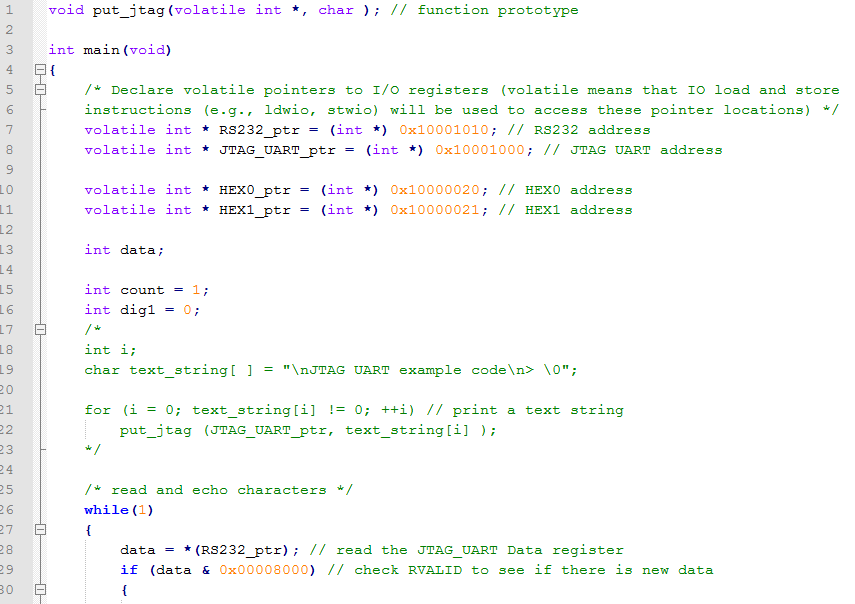
\includegraphics[width=\linewidth]{c1.png}
\end{Figure}

\begin{Figure}
 \centering
 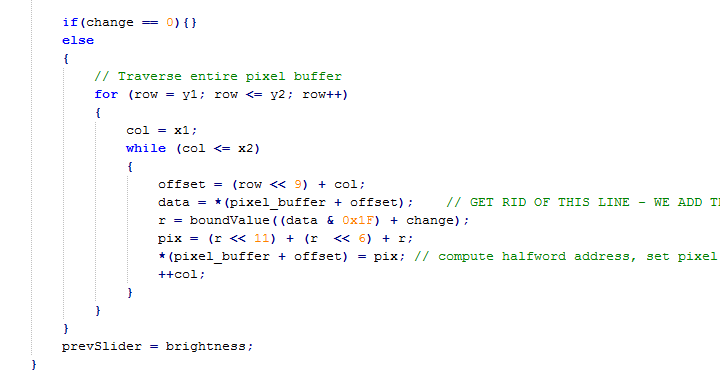
\includegraphics[width=\linewidth]{c2.png}
\end{Figure}

\begin{Figure}
 \centering
 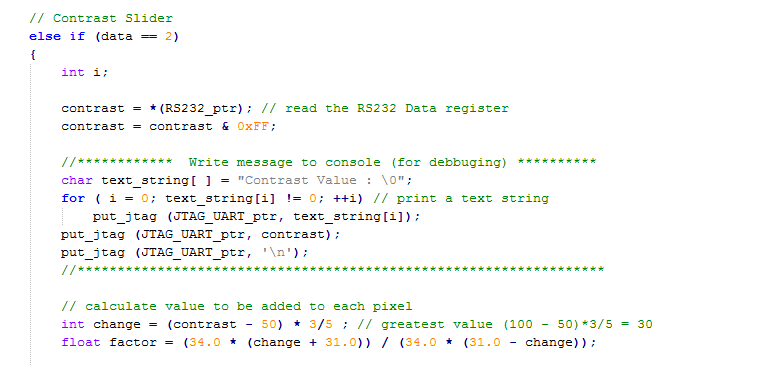
\includegraphics[width=\linewidth]{c3.png}
\end{Figure}

\begin{Figure}
 \centering
 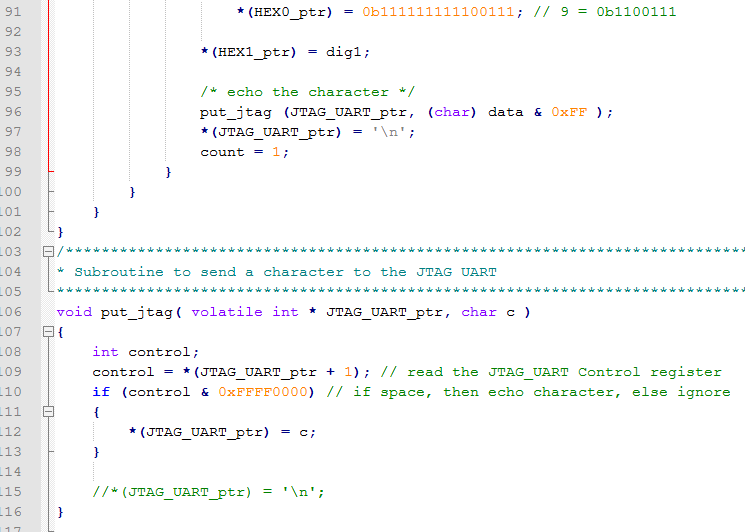
\includegraphics[width=\linewidth]{c4.png}
\end{Figure}


%----------------------------------------------------------------------------------------
\end{document}
